\begin{figure}
    \centering
    \begin{subfigure}{0.45\textwidth}
        \centering
        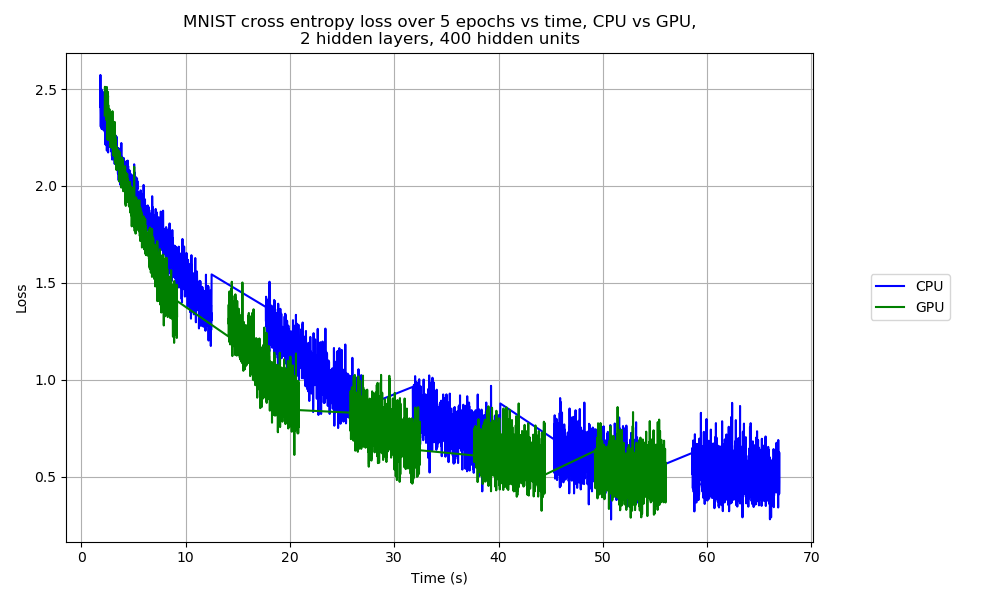
\includegraphics[width=\textwidth]{MNIST_cross_entropy_loss_over_5_epochs_vs_time,_CPU_vs_GPU,_2_hidden_layers,_400_hidden_units.png}
        \caption{Small model (2 hidden layers, 400 hidden units)}
        \label{fig:mnist small}
    \end{subfigure}
    \begin{subfigure}{0.45\textwidth}
        \centering
        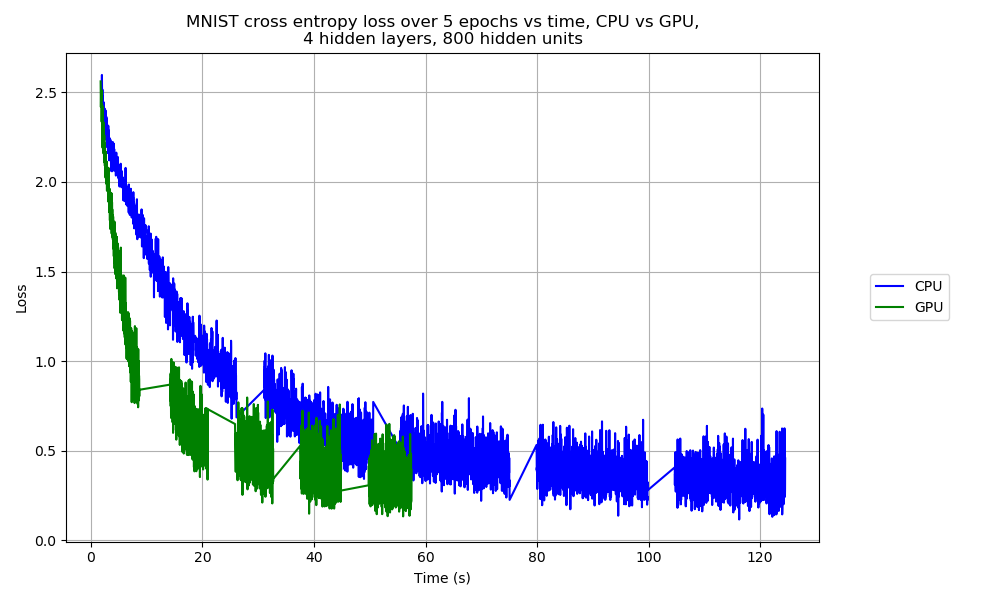
\includegraphics[width=\textwidth]{MNIST_cross_entropy_loss_over_5_epochs_vs_time,_CPU_vs_GPU,_4_hidden_layers,_800_hidden_units.png}
        \caption{Larger model (4 hidden layers, 800 hidden units)}
        \label{fig:mnist larger}
    \end{subfigure}
    \caption{Learning curves for different sized models trained on MNIST over 5 epochs, comparing training times between an Intel(R) Core(TM) i7-1065G7 CPU @ 1.30GHz and an NVIDIA GeForce MX250 GPU. Gaps in the training curves are due to evaluating test set accuracy once per epoch.}
    \label{fig:mnist cpu gpu}
\end{figure}
\begin{figure}
    \centering
    \begin{subfigure}{0.45\textwidth}
        \centering
        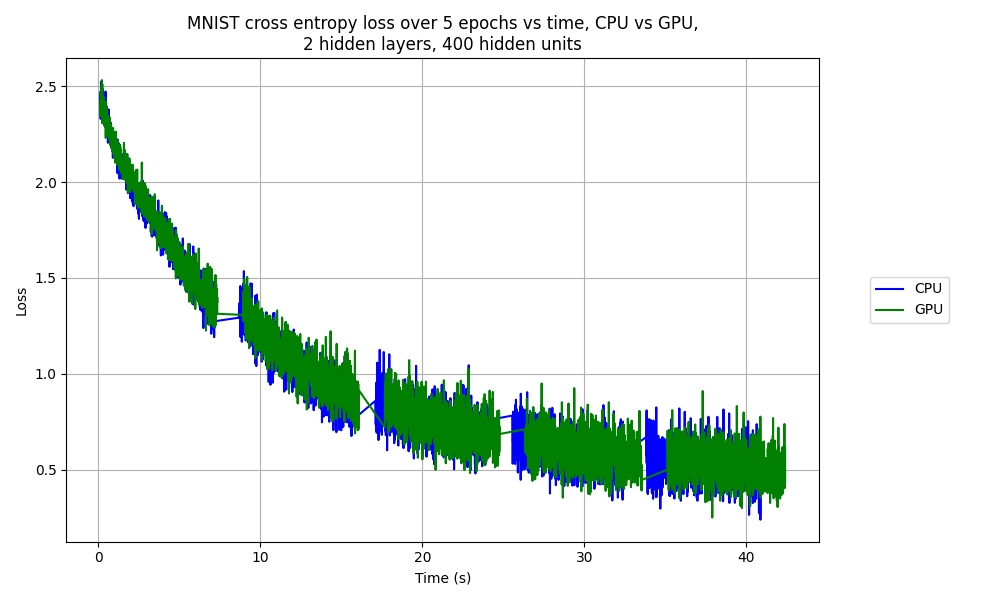
\includegraphics[width=\textwidth]{server_MNIST_cross_entropy_loss_over_5_epochs_vs_time,_CPU_vs_GPU,_2_hidden_layers,_400_hidden_units.png}
        \caption{Small model (2 hidden layers, 400 hidden units)}
        \label{fig:mnist small server}
    \end{subfigure}
    \begin{subfigure}{0.45\textwidth}
        \centering
        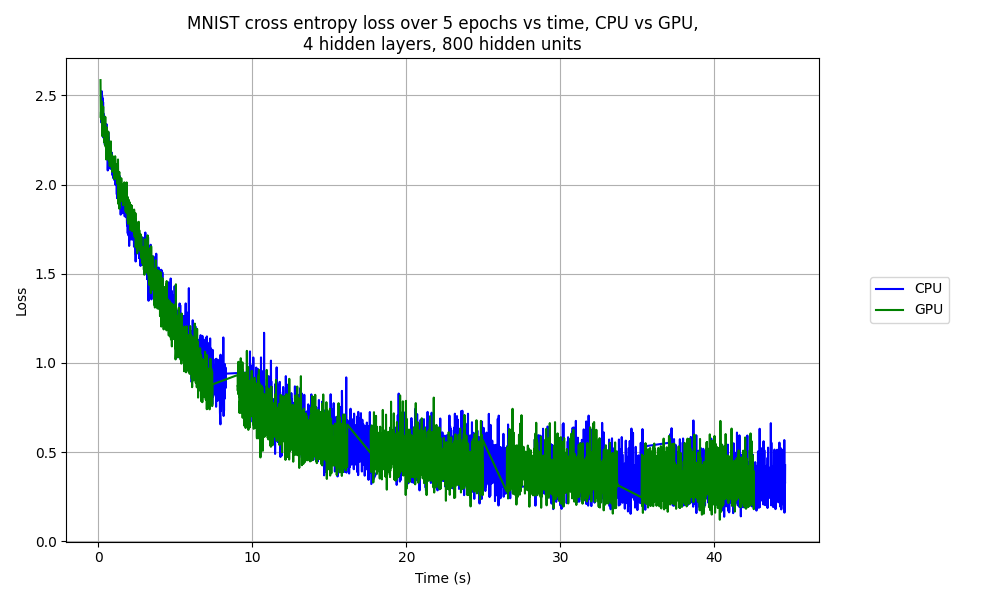
\includegraphics[width=\textwidth]{server_MNIST_cross_entropy_loss_over_5_epochs_vs_time,_CPU_vs_GPU,_4_hidden_layers,_800_hidden_units.png}
        \caption{Larger model (4 hidden layers, 800 hidden units)}
        \label{fig:mnist larger server}
    \end{subfigure}
    \caption{As for figure \ref{fig:mnist cpu gpu}, performed on a server with Intel(R) Xeon(R) Gold 5120 CPU @ 2.20GHz and NVIDIA TITAN V GPU}
    \label{fig:mnist cpu gpu server}
\end{figure}
\begin{figure}
    \centering
    \begin{subfigure}{0.45\textwidth}
        \centering
        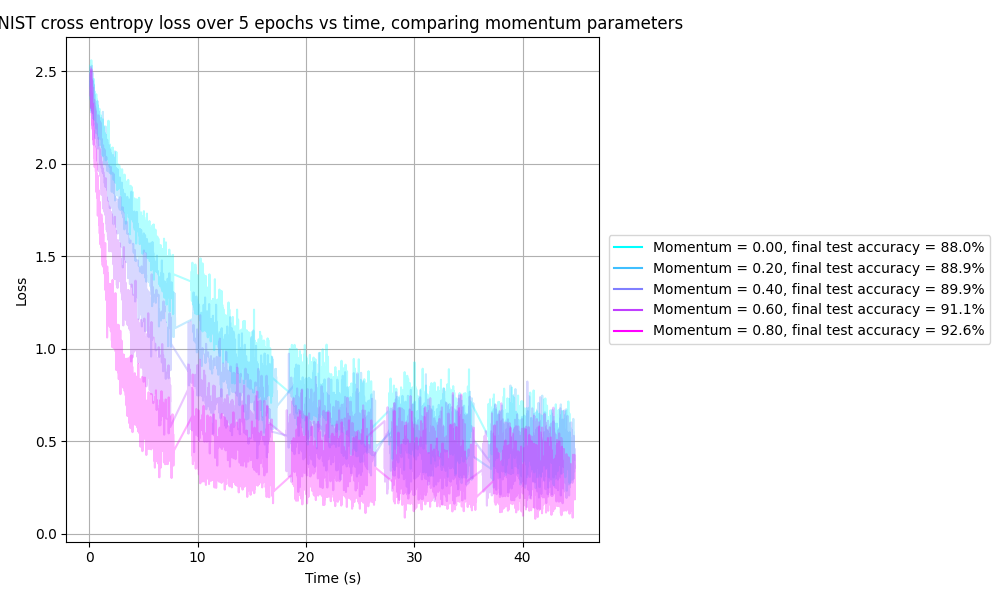
\includegraphics[width=\textwidth]{MNIST_cross_entropy_loss_over_5_epochs_vs_time,_comparing_momentum_parameters.png}
        \caption{Comparing momentum optimisation hyperparameter}
        \label{fig:mnist momentum}
    \end{subfigure}
    \begin{subfigure}{0.45\textwidth}
        \centering
        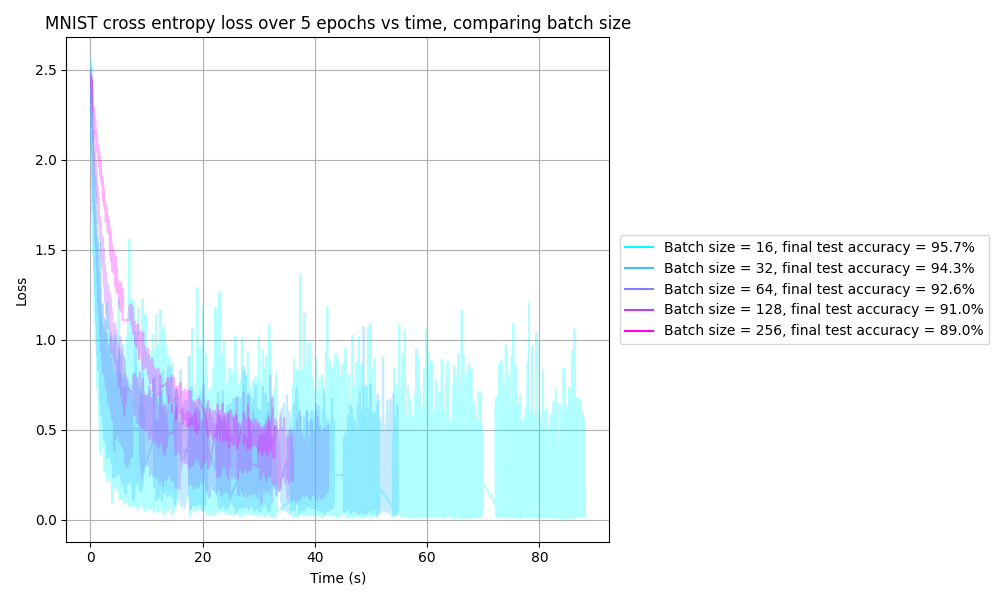
\includegraphics[width=\textwidth]{MNIST_cross_entropy_loss_over_5_epochs_vs_time,_comparing_batch_size.png}
        \caption{Comparing batch size}
        \label{fig:mnist batch size}
    \end{subfigure}
    \newline
    \begin{subfigure}{0.45\textwidth}
        \centering
        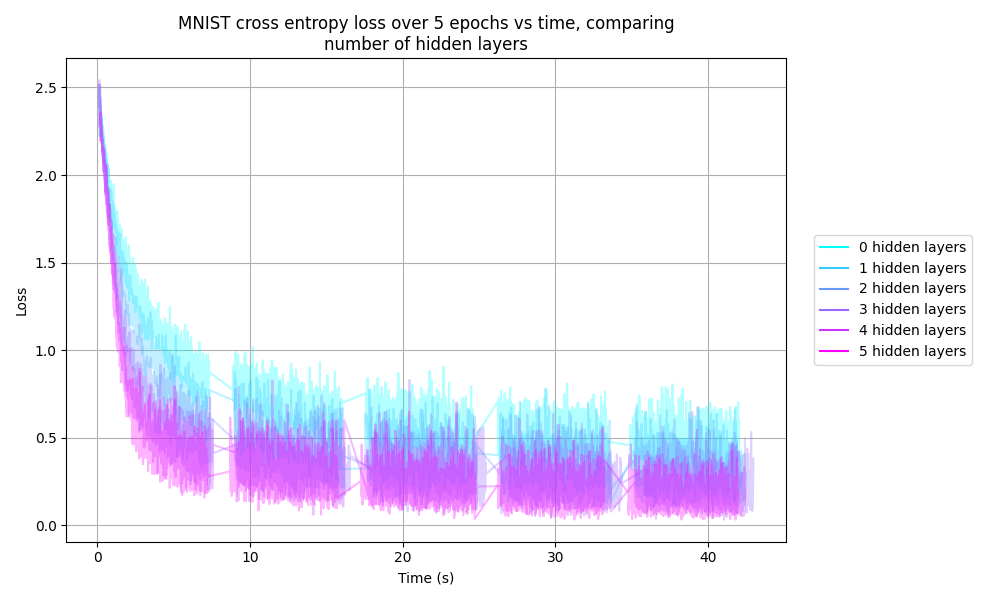
\includegraphics[width=\textwidth]{MNIST_cross_entropy_loss_over_5_epochs_vs_time,_comparing_number_of_hidden_layers.png}
        \caption{Comparing number of hidden layers}
        \label{fig:mnist num hidden layers}
    \end{subfigure}
    \begin{subfigure}{0.45\textwidth}
        \centering
        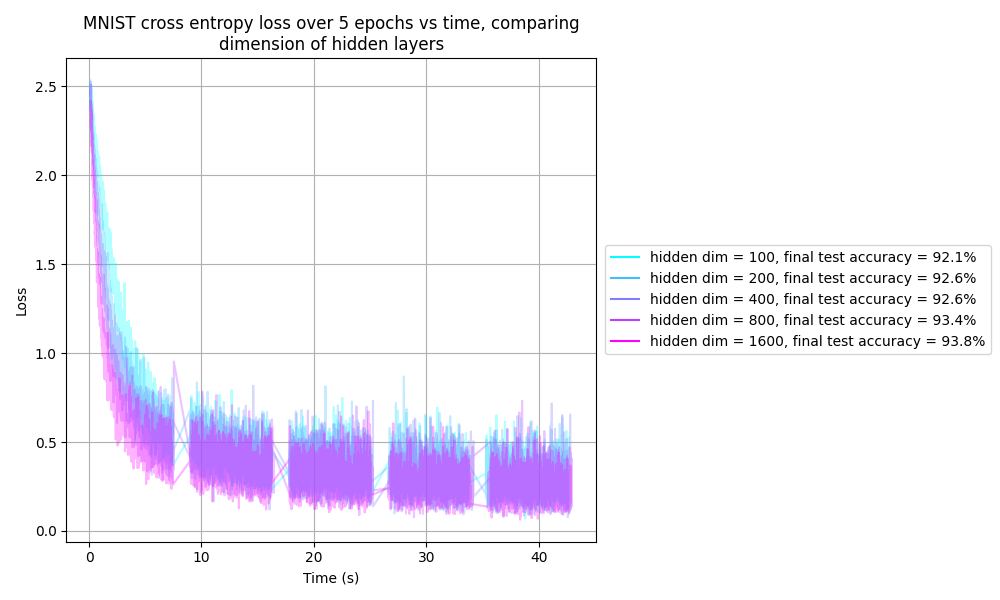
\includegraphics[width=\textwidth]{MNIST_cross_entropy_loss_over_5_epochs_vs_time,_comparing_dimension_of_hidden_layers.png}
        \caption{Comparing dimension of hidden layers}
        \label{fig:mnist hidden dimension}
    \end{subfigure}
    \newline
    \begin{subfigure}{0.45\textwidth}
        \centering
        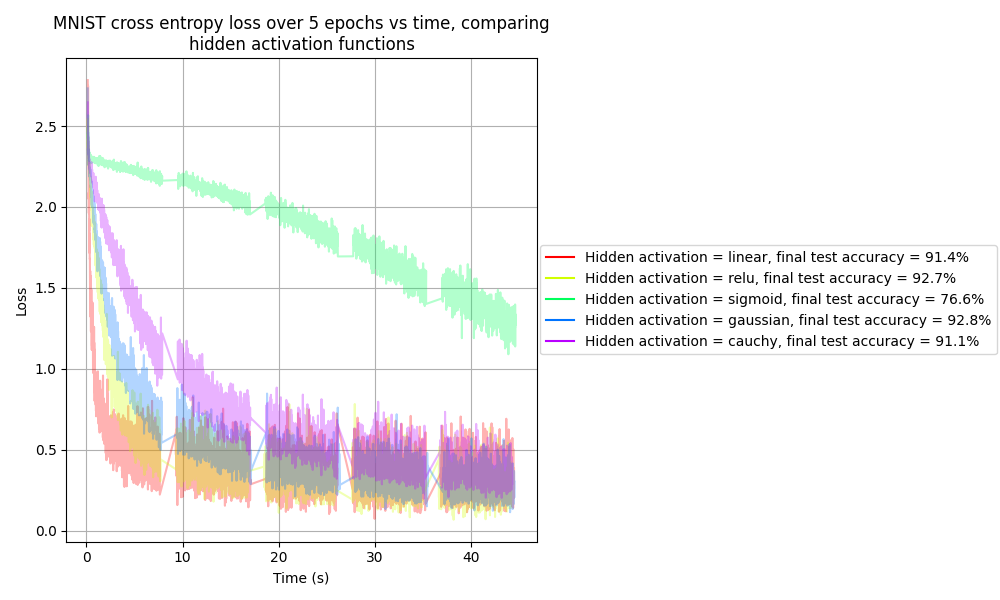
\includegraphics[width=\textwidth]{MNIST_cross_entropy_loss_over_5_epochs_vs_time,_comparing_hidden_activation_functions.png}
        \caption{Comparing hidden layer activation functions}
        \label{fig:mnist activation function}
    \end{subfigure}
    \caption{Comparing the effect of different hyperparameters on training a MLP on MNIST. Test set prediction accuracies are included in legends.}
    \label{fig:mnist parameters}
\end{figure}
\begin{figure}
    \centering
    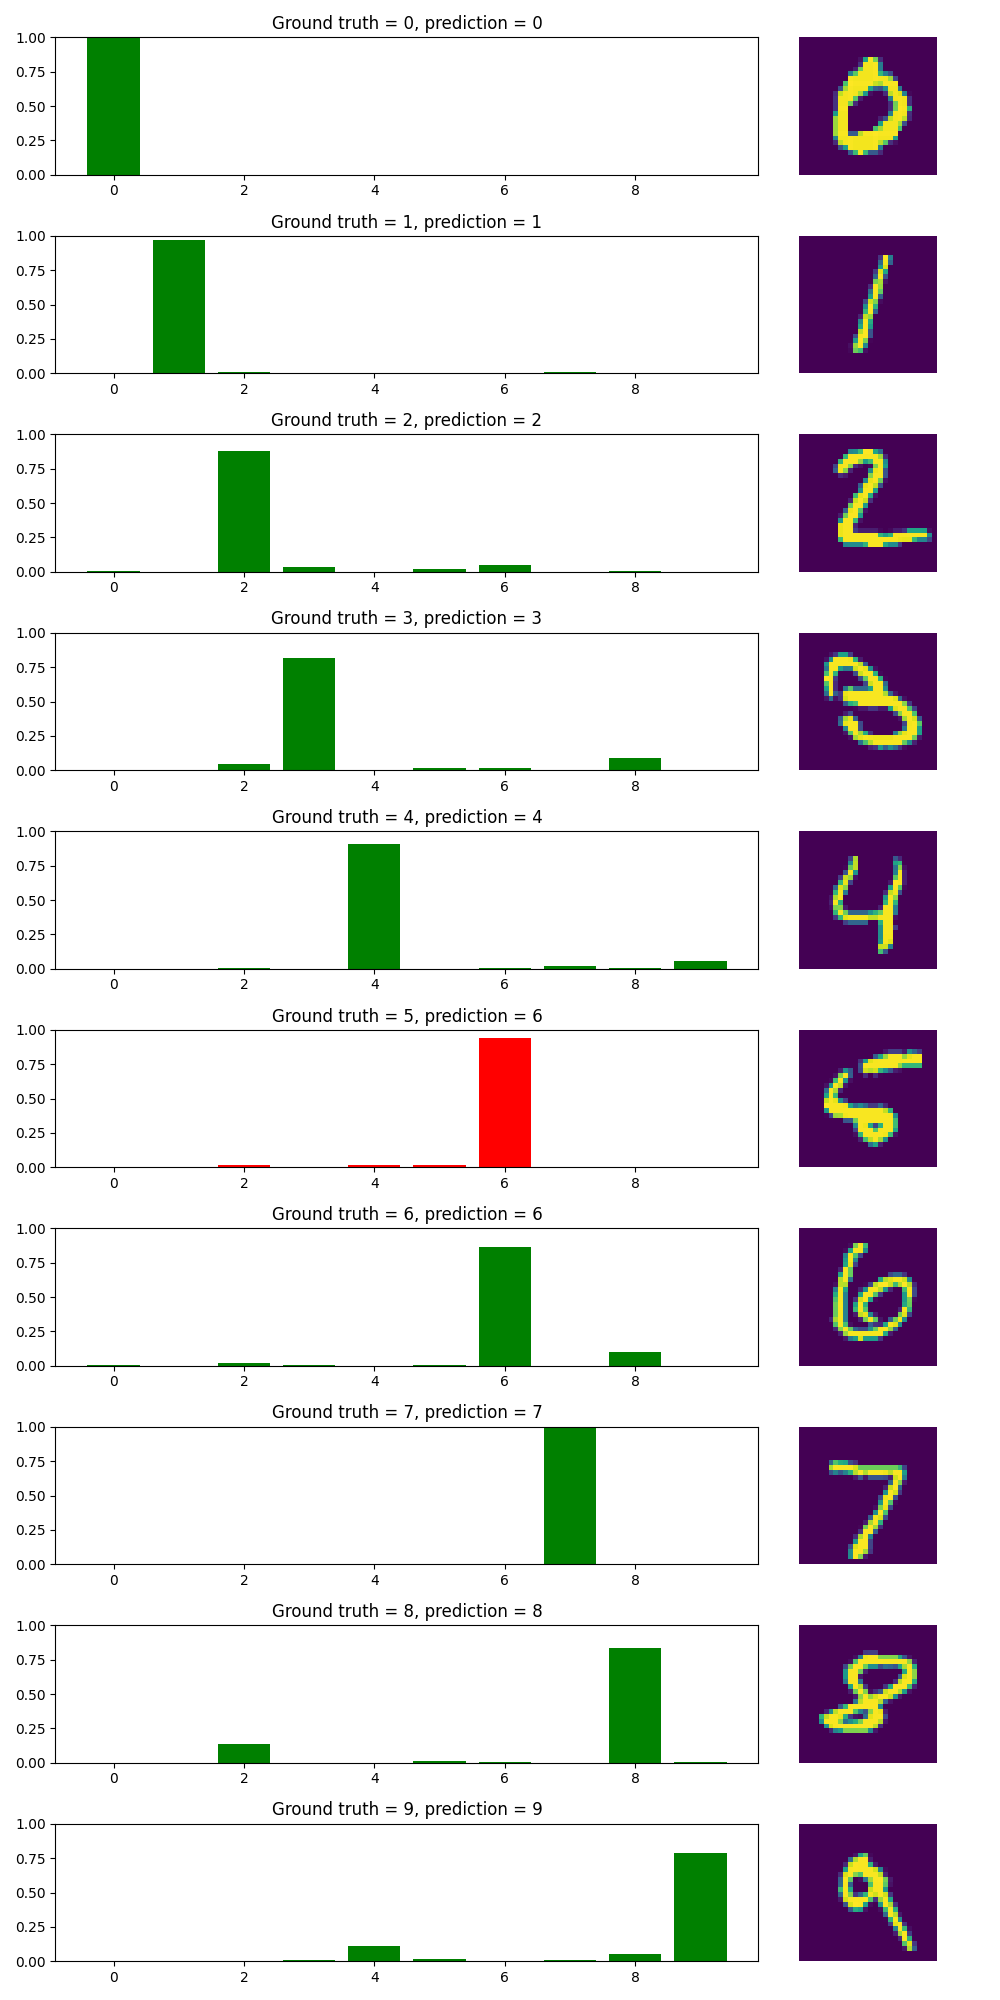
\includegraphics[width=0.6\textwidth]{Test_set_predictions.png}
    \caption{Predictions of a MLP trained on MNIST for 5 epochs on unseen examples of each digit from the test set}
    \label{fig:mnist predictions}
\end{figure}
